
\begin{center}
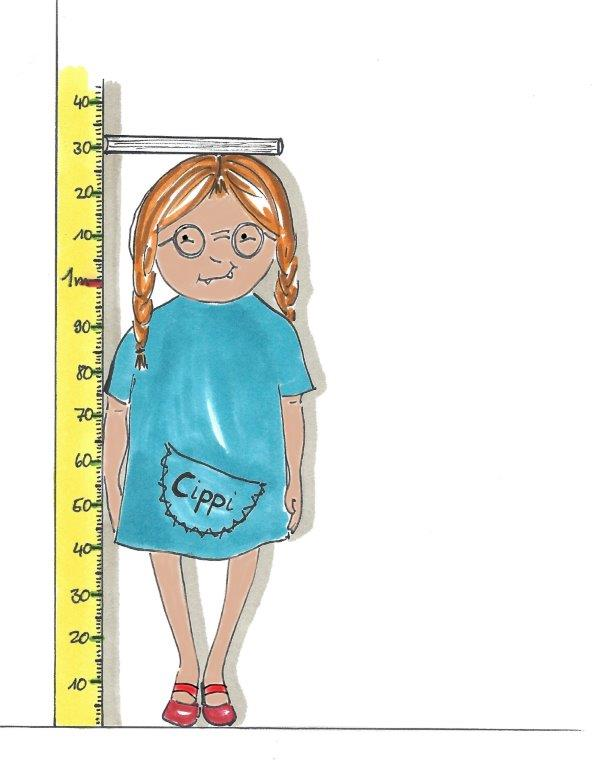
\includegraphics[width=0.6\textwidth]{content/3/chapter4/images/26.png}\\
Cippi measures how big she is
\end{center}

The three-way comparison operator <=> is often called the spaceship operator. The spaceship operator determines for two values A and B whether A < B, A == B, or A > B. You can define the spaceship operator or the compiler can autogenerates it for you.

To appreciate the advantages of the three-way comparison operator, let me start with the classical way of doing it.

\subsubsubsection{4.3.1\hspace{0.2cm} Ordering before C++20}

I implemented a simple int wrapper MyInt. Of course, I want to compare MyInt. Here is my solution using the function template isLessThan.

\noindent
MyInt supports less than comparisons
\begin{lstlisting}[style=styleCXX]
// comparisonOperator.cpp
#include <iostream>
struct MyInt {
	int value;
	explicit MyInt(int val): value{val} { }
	bool operator < (const MyInt& rhs) const {
		return value < rhs.value;
	}
};

template <typename T>
constexpr bool isLessThan(const T& lhs, const T& rhs) {
	return lhs < rhs;
}

int main() {
	std::cout << std::boolalpha << '\n';
	MyInt myInt2011(2011);
	MyInt myInt2014(2014);
	std::cout << "isLessThan(myInt2011, myInt2014): "
			  << isLessThan(myInt2011, myInt2014) << '\n';
	std::cout << '\n';
}
\end{lstlisting}

The program works as expected:

\begin{center}
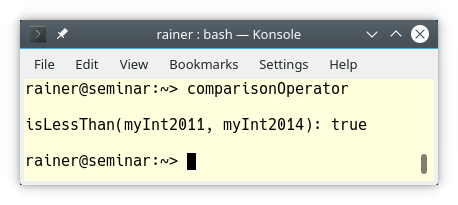
\includegraphics[width=0.6\textwidth]{content/3/chapter4/images/27.png}\\
Use of the less than operator
\end{center}

Honestly, MyInt is an unintuitive type. When you define one of the six ordering relations, you should define all of them. Intuitive types should be at least semiregular. Now, I have to write a lot of boilerplate code. Here are the missing five operators.

\noindent
The five missing comparison operators
\begin{lstlisting}[style=styleCXX]
bool operator == (const MyInt& rhs) const {
	return value == rhs.value;
}
bool operator != (const MyInt& rhs) const {
	return !(*this == rhs);
}
bool operator <= (const MyInt& rhs) const {
	return !(rhs < *this);
}
bool operator > (const MyInt& rhs) const {
	return rhs < *this;
}
bool operator >= (const MyInt& rhs) const {
	return !(*this < rhs);
}
\end{lstlisting}

Now, let’s jump to C++20 and the three-way comparison operator.

\subsubsubsection{4.3.2\hspace{0.2cm} Ordering since C++20}

You can define the three-way comparison operator or request it from the compiler with = default. In both cases you automatically get all six comparison operators: ==, !=, <, <=, >, and >=.

\noindent
Implement or request the three-way comparison operator
\begin{lstlisting}[style=styleCXX]
// threeWayComparison.cpp

#include <compare>
#include <iostream>

struct MyInt {
	int value;
	explicit MyInt(int val): value{val} { }
	auto operator<=>(const MyInt& rhs) const {
		return value <=> rhs.value;
	}
};

struct MyDouble {
	double value;
	explicit constexpr MyDouble(double val): value{val} { }
	auto operator<=>(const MyDouble&) const = default;
};

template <typename T>
constexpr bool isLessThan(const T& lhs, const T& rhs) {
	return lhs < rhs;
}

int main() {

	std::cout << std::boolalpha << '\n';
	
	MyInt myInt1(2011);
	MyInt myInt2(2014);
	
	std::cout << "isLessThan(myInt1, myInt2): "
	          << isLessThan(myInt1, myInt2) << '\n';
	
	MyDouble myDouble1(2011);
	MyDouble myDouble2(2014);
	
	std::cout << "isLessThan(myDouble1, myDouble2): "
	          << isLessThan(myDouble1, myDouble2) << '\n';
	
	std::cout << '\n';

}
\end{lstlisting}

The user-defined (line 9) and the compiler-generated (line 17) three-way comparison operators work as expected.

\begin{center}
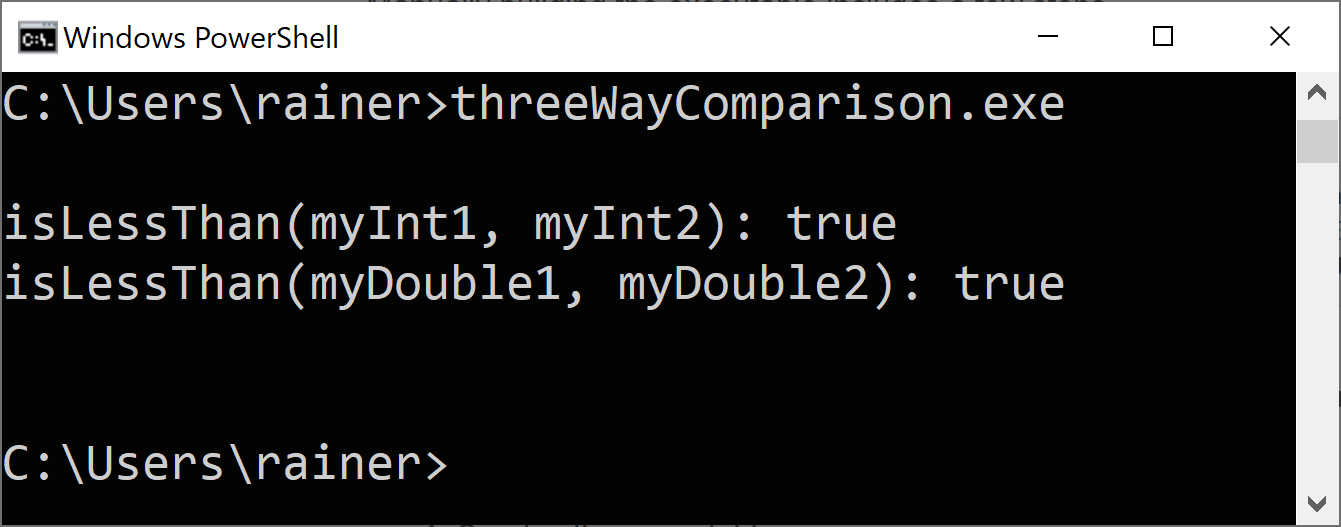
\includegraphics[width=0.6\textwidth]{content/3/chapter4/images/28.png}\\
Use of the user-defined and compiler-generated spaceship operator
\end{center}

In this case, there are a few subtle differences between the user-defined and the compiler-generated three-way comparison operator. The compiler-deduced return type for MyInt (line 9) supports strong ordering, and the compiler-deduced return type of MyDouble (line 17) supports partial ordering.

\begin{tcolorbox}[colback=red!5!white,colframe=red!75!black,title=Automatic Comparision of Pointers]

The compiler-generated three-way comparison operator compares the pointers but not the referenced objects.

\noindent
Automatic Comparison of Pointers
\begin{lstlisting}[style=styleCXX]
// spaceshipPoiner.cpp

#include <iostream>
#include <compare>
#include <vector>

struct A {
	std::vector<int>* pointerToVector;
	auto operator <=> (const A&) const = default;
};

int main() {

	std::cout << '\n';
	
	std::cout << std::boolalpha;
	
	A a1{new std::vector<int>()};
	A a2{new std::vector<int>()};
	
	std::cout << "(a1 == a2): " << (a1 == a2) << "\n\n";

}
\end{lstlisting}

Astonighly, the result of a1 == a2 (line 21) is false and not true, because the adresses of std::vector<int>* are compared.

\begin{tcblisting}{commandshell={}}
(a1 == a2): false
\end{tcblisting}

\begin{center}
Comparison of pointers
\end{center}

\end{tcolorbox}

There are three comparison categories.

\subsubsubsection{4.3.3\hspace{0.2cm} Comparision Categories}

The names of the three comparison categories are strong ordering, weak ordering, and partial ordering. For a type T, the three following properties distinguish the three comparison categories.

\begin{enumerate}
\item 
T supports all six relational operators: ==, !=, <, <=, >, and >= (short: Relational Operator)

\item 
All equivalent values are indistinguishable: (short: Equivalence)

\item 
All values of T are comparable: For arbitrary values a and b of T, one of the three relations a < b, a == b , and a > b must be true (short: Comparable)
\end{enumerate}

When you use as a sorting criterion the case-insensitive representation of a string, equivalent values need not be different. Additionally, two arbitrary floating-point values need not to be comparable: for a = 5.5, and b = NaN (Not a Number) neither of the following expressions returns true: a < Nan, a == Nan , or a > Nan.

Based on the three properties, distinguishing the three comparison strategies is straightforward:

\begin{center}
Strong, weak, and partial ordering
\end{center}

\begin{table}[H]
\centering
\begin{tabular}{llll}
Comparison Category & Relational Operator & Equivalence & Comparable \\ \hline
Strong Ordering     & yes                 & yes         & yes        \\
Weak Ordering       & yes                 &             & yes        \\
Partial Ordering    & yes                 &             &           
\end{tabular}
\end{table}


A type supporting strong ordering supports implicitly weak and partial ordering. The same holds for weak ordering. A type supporting weak ordering also supports partial ordering. The other directions do not apply.

\begin{center}
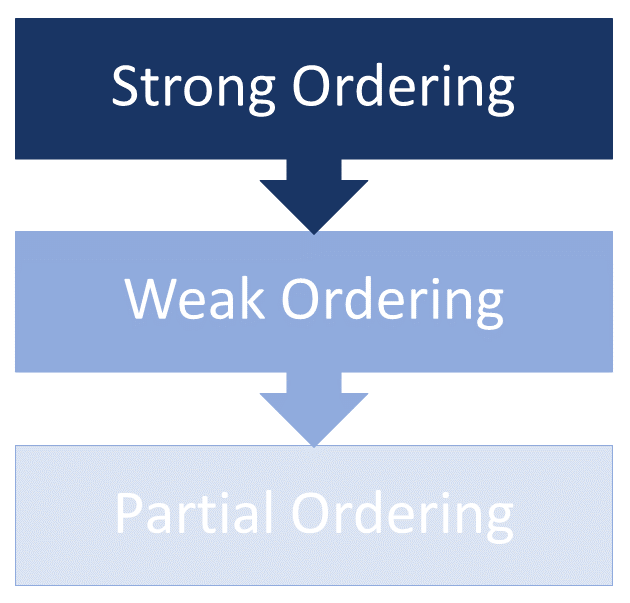
\includegraphics[width=0.6\textwidth]{content/3/chapter4/images/29.png}\\
Strong, weak, and partial ordering
\end{center}

If the declared return type is auto, then the actual return type is the common comparison category of the base and member subobject and the member array elements to be compared.

Let me give you an example for this rule:

\noindent
Implement or request the three-way comparison operator
\begin{lstlisting}[style=styleCXX]
// strongWeakPartial.cpp

#include <compare>

struct Strong {
	std::strong_ordering operator <=> (const Strong&) const = default;
};

struct Weak {
	std::weak_ordering operator <=> (const Weak&) const = default;
};

struct Partial {
	std::partial_ordering operator <=> (const Partial&) const = default;
};

struct StrongWeakPartial {

	Strong s;
	Weak w;
	Partial p;
	
	auto operator <=> (const StrongWeakPartial&) const = default;
	
	// FINE
	// std::partial_ordering operator <=> (const StrongWeakPartial&) const = default\
	;
	
	// ERROR
	// std::strong_ordering operator <=> (const StrongWeakPartial&) const = default;\
	
	// std::weak_ordering operator <=> (const StrongWeakPartial&) const = default; \


};

int main() {

	StrongWeakPartial a1, a2;
	
	a1 < a2;

}
\end{lstlisting}

he type StrongWeakPartial has subtypes supporting strong (line 6), weak (line 10), and partial ordering (line 14). The common comparison category for the type StrongWeakPartial (line 17) is, therefore, std::partial\_ordering. Using a more powerful comparison category, such as strong ordering (line 29) or weak ordering (line 30), would result in a compile-time error.

Now, I want to focus on the compiler-generated spaceship operator.

\subsubsubsection{4.3.4\hspace{0.2cm} The Compiler-Generated Spaceship Operator}

The compiler-generated three-way comparison operator needs the header <compare>, is implicitly constexpr and \href{https://www.modernescpp.com/index.php/c-core-guidelines-the-noexcept-specifier-and-operator}{noexcept}, and performs a lexicographical comparison.

You can even directly use the three-way comparison operator.

\noindent
4.3.4.1\hspace{0.2cm} Direct Use of the Three-Way Comparison Operator

The program spaceship.cpp directly uses the spaceship operator.

\noindent
Implement or request the three-way comparison operator
\begin{lstlisting}[style=styleCXX]
// spaceship.cpp

#include <compare>
#include <iostream>
#include <string>
#include <vector>

int main() {
	
	std::cout << '\n';
	
	int a(2011);
	int b(2014);
	auto res = a <=> b;
	if (res < 0) std::cout << "a < b" << '\n';
	else if (res == 0) std::cout << "a == b" << '\n';
	else if (res > 0) std::cout << "a > b" << '\n';
	
	std::string str1("2014");
	std::string str2("2011");
	auto res2 = str1 <=> str2;
	if (res2 < 0) std::cout << "str1 < str2" << '\n';
	else if (res2 == 0) std::cout << "str1 == str2" << '\n';
	else if (res2 > 0) std::cout << "str1 > str2" << '\n';
	
	std::vector<int> vec1{1, 2, 3};
	std::vector<int> vec2{1, 2, 3};
	auto res3 = vec1 <=> vec2;
	if (res3 < 0) std::cout << "vec1 < vec2" << '\n';
	else if (res3 == 0) std::cout << "vec1 == vec2" << '\n';
	else if (res3 > 0) std::cout << "vec1 > vec2" << '\n';
	
	std::cout << '\n';

}
\end{lstlisting}

The program uses the spaceship operator for int (line 14), string (line 21), and vector (line 28). Here is the output of the program.

\begin{tcblisting}{commandshell={}}
a < b
str1 > str2
vec1 == vec2
\end{tcblisting}

\begin{center}
Direct use of the spaceship operator
\end{center}

As already mentioned, these comparisons are constexpr and could be done at compile time.

\noindent
4.3.4.2\hspace{0.2cm} Comparison at Compile Time

The three-way comparison operator is implicitly constexpr. Consequently, I can simplify the previous program threeWayComparison.cpp and compare MyDouble in the following program at compile time.

\noindent
A compiler-generated constexpr three-way comparison operator
\begin{lstlisting}[style=styleCXX]
// threeWayComparisonAtCompileTime.cpp

#include <compare>
 #include <iostream>

struct MyDouble {
	 double value;
	 explicit constexpr MyDouble(double val): value{val} { }
	 auto operator<=>(const MyDouble&) const = default;
};

 template <typename T>
 constexpr bool isLessThan(const T& lhs, const T& rhs) {
	 return lhs < rhs;
}

 int main() {
	
	std::cout << std::boolalpha << '\n';
	
	constexpr MyDouble myDouble1(2011);
	constexpr MyDouble myDouble2(2014);
	
	constexpr bool res = isLessThan(myDouble1, myDouble2);
	
	std::cout << "isLessThan(myDouble1, myDouble2): "
	<< res << '\n';
	
	std::cout << '\n';

}
\end{lstlisting}

I ask for the result of the comparison at compile time (line 24), and I get it.

\begin{center}
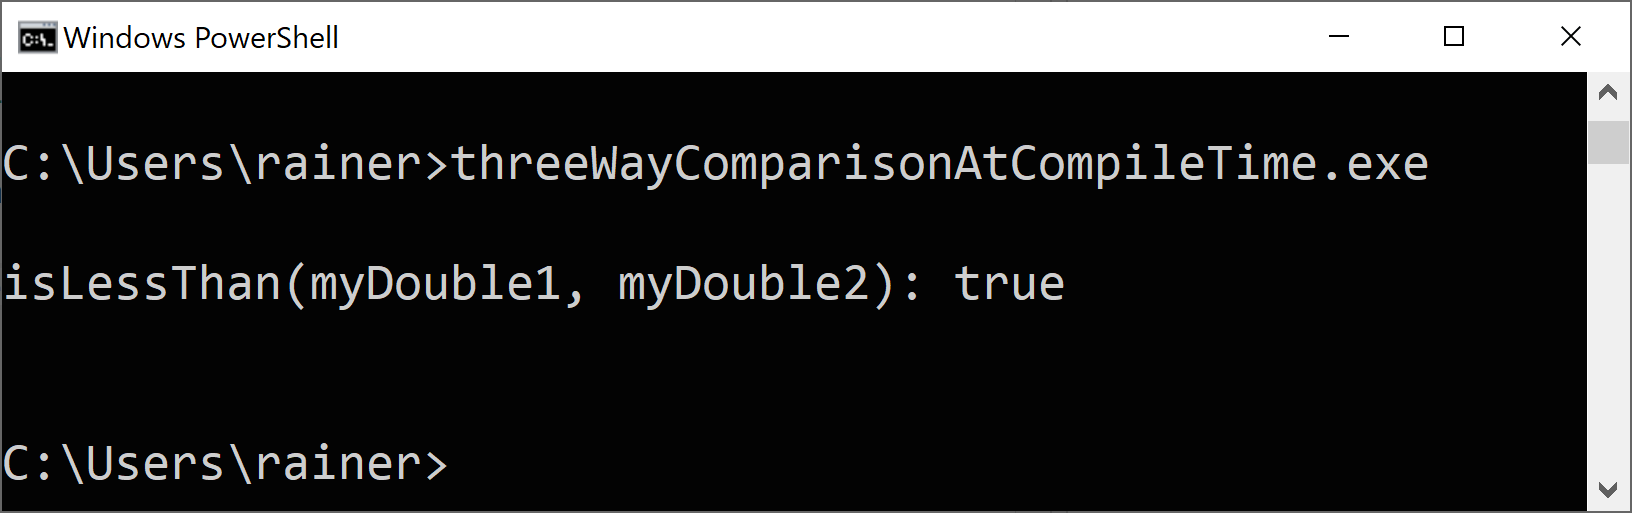
\includegraphics[width=0.6\textwidth]{content/3/chapter4/images/30.png}\\
Use of the constexpr compiler-generated spaceship operator
\end{center}

\noindent
4.3.4.3\hspace{0.2cm} Direct Use of the Three-Way Comparison Operator



The compiler-generated three-way comparison operator performs a lexicographical comparison. Lexicographical comparison, in this case, means that all base classes are compared left to right and all non-static members of the class in their declaration order. I have to qualify: for performance reasons, the compiler-generated == and != operator behave differently in C++20. I will write about this exception in the section for the optimized == and != operators.

The post \href{https://devblogs.microsoft.com/cppblog/simplify-your-code-with-rocket-science-c20s-spaceship-operator/}{“Simplify Your Code With Rocket Science: C++20’s Spaceship Operator”} from the Microsoft C++ Team Blog provides an impressive example of lexicographical comparison. For readability, I added a few comments.

\noindent
Lexicographical comparison
\begin{lstlisting}[style=styleCXX]
struct Basics {
	 int i;
	 char c;
	 float f;
	 double d;
	 auto operator<=>(const Basics&) const = default;
};

struct Arrays {
	 int ai[1];
	 char ac[2];
	 float af[3];
	 double ad[2][2];
	 auto operator<=>(const Arrays&) const = default;
};

 struct Bases : Basics, Arrays {
	 auto operator<=>(const Bases&) const = default;
};

int main() {
	constexpr Bases a = { { 0, 'c', 1.f, 1. }, // Basics
	 					{ { 1 }, { 'a', 'b' }, { 1.f, 2.f, 3.f }, // Arrays
						{ { 1., 2. }, { 3., 4. } } } };
	constexpr Bases b = { { 0, 'c', 1.f, 1. }, // Basics
	 					{ { 1 }, { 'a', 'b' }, { 1.f, 2.f, 3.f }, // Arrays
		 				{ { 1., 2. }, { 3., 4. } } } };
	static_assert(a == b);
	static_assert(!(a != b));
	static_assert(!(a < b));
	static_assert(a <= b);
	static_assert(!(a > b));
	static_assert(a >= b);
}
\end{lstlisting}

I assume the most challenging aspect of the program is not the spaceship operator, but the initialization of Bases via aggregate initialization (lines 22 and 25). Aggregate initialization enables us to directly initialize the members of a class type (class, struct, union) when the members are all public. In this case, you can use brace initialization. Aggregate initialization is discussed in more detail in the section on designated initializers in C++20.

\begin{tcolorbox}[colback=blue!5!white,colframe=blue!75!black,title={Optimized == and != Operators}]

There is an optimization potential for a string-like or vector-like types. In this case, a == and != may be faster than the compiler-generated three-way comparison operator. The == and != operators can stop if the two values compared have different lengths. Otherwise, if one value were a prefix of the other, lexicographical comparison would compare all elements until the end of the shorter value. The standardization committee was aware of this performance issue and fixed it with the paper \href{http://www.open-std.org/jtc1/sc22/wg21/docs/papers/2019/p1185r2.html}{P1185R2}. Consequently, the compiler-generated == and != operators compare, in the case of a string-like or a vector-like type, first their lengths and then their content if necessary.

\end{tcolorbox}

Now, it’s time for something new in C++. C++20 introduces the concept of rewriting expressions.

\subsubsubsection{4.3.5\hspace{0.2cm} Rewriting Expressions}

When the compiler sees something such as a < b, it rewrites it to (a <=> b) < 0 using the spaceship operator.

Of course, the rule applies to all six comparison operators: a OP b becomes (a <=> b) OP 0. It’s even better. If there is no conversion of the type(a) to type(b), the compiler generates the new expression 0 OP (b <=> a).

For example, this means for the less-than operator, if (a <=> b) < 0 does not work, the compiler generates 0 < (b <=> a). In essence, the compiler takes care of the symmetry of the comparison operators.

Here are a few examples of rewriting expressions:

\noindent
Rewriting expressions with MyInt
\begin{lstlisting}[style=styleCXX]
// rewritingExpressions.cpp

#include <compare>
#include <iostream>

class MyInt {
public:
	 constexpr MyInt(int val): value{val} { }
	 auto operator<=>(const MyInt& rhs) const = default;
private:
	 int value;
};

int main() {
	
	std::cout << '\n';
	
	constexpr MyInt myInt2011(2011);
	constexpr MyInt myInt2014(2014);
	
	constexpr int int2011(2011);
	constexpr int int2014(2014);
	
	if (myInt2011 < myInt2014) std::cout << "myInt2011 < myInt2014" << '\n';
	if ((myInt2011 <=> myInt2014) < 0) std::cout << "myInt2011 < myInt2014" << '\n';
	
	std::cout << '\n';
	
	if (myInt2011 < int2014) std:: cout << "myInt2011 < int2014" << '\n';
	if ((myInt2011 <=> int2014) < 0) std:: cout << "myInt2011 < int2014" << '\n';
	
	std::cout << '\n';
	
	if (int2011 < myInt2014) std::cout << "int2011 < myInt2014" << '\n';
	if (0 < (myInt2014 <=> int2011)) std:: cout << "int2011 < myInt2014" << '\n';
	
	std::cout << '\n';

}
\end{lstlisting}

I used in line 24, line 29, and line 34 the less-than operator and the corresponding spaceship expression. Line 35 is the most interesting one. It exemplifies how the comparison (int2011 < myInt2014) triggers the generation of the spaceship expression (0 < (myInt2014 <=> int2011).

\begin{tcblisting}{commandshell={}}
myInt2011 < myInt2014
myInt2011 < myInt2014

myInt2011 < int2014
myInt2011 < int2014

int2011 < myInt2014
int2011 < myInt2014
\end{tcblisting}

\begin{center}
Rewriting expressions
\end{center}

Honestly, MyInt has an issue: its constructor taking one argument should be declared explicit. Constructors taking one argument such as MyInt(int val) (line 8) are conversion constructors. This means that an instance from MyInt can be generated from any integral or floating-point value because each integral or floating-point value can implicitly be converted to an int.

Let me fix this issue and make the constructor MyInt(int val) explicit. To support the comparison of MyInt and int, MyInt needs an additional three-way comparison operator for int.

\noindent
An additional three-way comparison operator for int
\begin{lstlisting}[style=styleCXX]
// threeWayComparisonForInt.cpp

#include <compare>
#include <iostream>

class MyInt {
public:
	constexpr explicit MyInt(int val): value{val} { }
	
	auto operator<=>(const MyInt& rhs) const = default;
	
	constexpr auto operator<=>(const int& rhs) const {
		return value <=> rhs;
	}
private:
	int value;
};

template <typename T, typename T2>
constexpr bool isLessThan(const T& lhs, const T2& rhs) {
	return lhs < rhs;
}

int main() {

	std::cout << std::boolalpha << '\n';
	
	constexpr MyInt myInt2011(2011);
	constexpr MyInt myInt2014(2014);
	
	constexpr int int2011(2011);
	constexpr int int2014(2014);
	
	std::cout << "isLessThan(myInt2011, myInt2014): "
	<< isLessThan(myInt2011, myInt2014) << '\n';
	
	std::cout << "isLessThan(int2011, myInt2014): "
	<< isLessThan(int2011, myInt2014) << '\n';
	
	std::cout << "isLessThan(myInt2011, int2014): "
	<< isLessThan(myInt2011, int2014) << '\n';
	
	constexpr auto res = isLessThan(myInt2011, int2014);
	
	std::cout << '\n';

}
\end{lstlisting}

I defined in (line 10) the three-way comparison operator and declared it constexpr. The user-defined three-way comparison operator is not implicitly constexpr, unlike the compiler-generated threeway comparison operator. The comparison of MyInt and int is possible in each combination (lines 34, 37, and 40).

\begin{tcblisting}{commandshell={}}
isLessThan(MyInt2011, myInt2014): true
isLessThan(int2011, myInt2014): true
isLessThan(MyInt2011, int2014): true
\end{tcblisting}

\begin{center}
Three-way comparison operator for int
\end{center}

Honestly, the implementation of the various three-way comparison operators is very elegant. The compiler auto-generates the comparison of MyInt, and the user defines the comparison with int explicitly. Additionally, thanks to reordering, you have to define only 2 operators to get 18 = 3 * 6 combinations of comparison operators. The 3 stands for the combinations int OP MyInt, MyInt OP MyInt, and MyInt OP int and the 6 for six comparison operators.

\subsubsubsection{4.3.6\hspace{0.2cm} User-Defined and Auto-Generated Comparison Operators}

When you can define one of the six comparison operators and also auto-generate all of them using the spaceship operator, there is one question: Which one has the higher priority? For example, this implementation MyInt has a user-defined less-than-and-equal-to operator and also the compilergenerated six comparison operators.

Let’s see what happens.

\noindent
The interplay of user-defined and auto-generated operators
\begin{lstlisting}[style=styleCXX]
// userDefinedAutoGeneratedOperators.cpp

#include <compare>
#include <iostream>

class MyInt {
public:
	constexpr explicit MyInt(int val): value{val} { }
	bool operator == (const MyInt& rhs) const {
	std::cout << "== " << '\n';
		return value == rhs.value;
	}
	bool operator < (const MyInt& rhs) const {
	std::cout << "< " << '\n';
		return value < rhs.value;
	}
	
	auto operator<=>(const MyInt& rhs) const = default;

private:
	int value;
};

int main() {

	MyInt myInt2011(2011);
	MyInt myInt2014(2014);
	
	myInt2011 == myInt2014;
	myInt2011 != myInt2014;
	myInt2011 < myInt2014;
	myInt2011 <= myInt2014;
	myInt2011 > myInt2014;
	myInt2011 >= myInt2014;

}
\end{lstlisting}

To see the user-defined == and < operator in action, I write a corresponding message to std::cout. Neither operator can be constexpr, because std::cout is a run-time operation.

Let’s see what happens:

\begin{tcblisting}{commandshell={}}
==
==
<
\end{tcblisting}

\begin{center}
User-defined and auto-generated operators
\end{center}

In this case, the compiler uses the user-defined == (lines 29 and 30) and < operators (line 31). Additionally, the compiler synthesizes the != operator (line 30) out of the == operator. On the other hand, the compiler does not synthesize the == operator out of the != operator.

\begin{tcolorbox}[colback=blue!5!white,colframe=blue!75!black,title={Similarity to Python}]
In Python 3, the compiler generates != out of == if necessary but not the other way around. In Python 2, the so-called rich comparison (the user-defined six comparison operators) has higher priority than Python’s three-way comparison operator \_\_cmp\_\_. I have to say Python 2 because the three-way comparison operator \_\_cmp\_\_ was removed in Python 3.	
\end{tcolorbox}	

\begin{tcolorbox}[colback=mygreen!5!white,colframe=mygreen!75!black,title={Distilled Information}]
\begin{itemize}
\item 
By defaulting the operator <=>, the compiler autogenerates the six comparison operators. The compiler-generated comparison operators apply lexicographical comparison: all base classes are compared left to right and all non-static members of the class in their declaration order.

\item 
When auto-generated comparison operators and user-defined comparison operators are both present, the user-defined comparison operators have a higher priority.

\item 
The compiler rewrites expressions to take care of the symmetry of the comparison operators. For example if (a <=> b) < 0 does not work, the compiler generates 0 < (b <=> a).
\end{itemize}
\end{tcolorbox}	
























